\documentclass[article]{jss}
\usepackage[utf8]{inputenc}

\providecommand{\tightlist}{%
  \setlength{\itemsep}{0pt}\setlength{\parskip}{0pt}}

\author{
Derek Corcoran\\University of Missouri \And Elisabeth Webb\\University of Missouri, USGS \And Dylan Kesler\\Institute Of Bird Population
}
\title{Selecting priority areas from diversity and individual species abundance
\pkg{DiversityOccupancy}}
\Keywords{\pkg{DiversityOccupancy}, Occupancy Modeling, \proglang{R}}

\Abstract{
Lately occupancy modeling has been vastly used as a tool for ecological
research and management planing. However mostly it is used by
interpreting single species models. We present the
\pkg{DiversityOccupancy} in the \proglang{R} environment. The objective
of this package is to simultaneously model factors associated with
occupancy and abundance of individual species using a detection history
file, and to use predicted abundances to calculate species diversity for
each sampling site. The package then models factor(s) associated with
among-site species diversity, which can then be combined with spatial
data to identify areas that contain both high abundance of species of
conservation concern and high species diversity.
}

\Plainauthor{Derek Corcoran, Elisabeth Webb, Dylan Kesler}
\Shorttitle{\pkg{DiversityOccupancy}: Selecting Priority Areas}
\Plainkeywords{keywords, not capitalized, Occupancy modeling}

%% publication information
%% \Volume{50}
%% \Issue{9}
%% \Month{June}
%% \Year{2012}
\Submitdate{}
%% \Acceptdate{2012-06-04}

\Address{
    Derek Corcoran\\
  University of Missouri\\
  First line Second line\\
  E-mail: \href{mailto:corcoranbarriosd@missouri.edu}{\nolinkurl{corcoranbarriosd@missouri.edu}}\\
  URL: \url{http://rstudio.com}\\~\\
      }

\usepackage{amsmath}

\begin{document}

\section{Introduction}\label{introduction}

\subsection{Single-species or multiple-species
management}\label{single-species-or-multiple-species-management}

The ecological and management literature has usually valued the idea of
managing for diversity. This, however clashes with the classic way in
which conservation takes place. Conservation agencies, goverments,
scientists and international organizations such as International Union
for Conservation of Nature (IUCN), classify species according to a
conservation status, and policies are made to safeward the ones that are
envisioned as species of conservation concerned
\citep{keller2004red, rodrigues2006value}. Single species are easier to
manage for, and it is easier to keep track the status of a species than
it is to define management for diversity
\citep{simberloff1998flagships}, it is also more complicated to sample
to keep track of changes in diversity.

There are several aproaches to design management meassures based on
single species, such as using umbrella species
\citep{crosby2015looking, bichet2016maintaining}, Habitat Suitability
Indices (HSI)
\citep{reza2013integrating, soniat2013predicting, zohmann2013modelling},
Species distribution modeling (SDM)
\citep{peterson2011ecological, guisan2013predicting}. Even when the
literature mostly criticizes the use of such aproaches due to the
ineffectiveness in preventing loss of biodiversity
\citep{roberge2004usefulness, branton2011assessing}

One of the problems of managing simple species, is that is usually very
difficult to predict what will happend to other species and because of
that it is hard to predict what will happend to diversity
\citep{pulliam2000relationship}, with some examples showing that even
management meassurements that use some species as umbrella species for
conservation of ecosystems leading to undesired community effects
\citep{white2013conservation}.

Managing for multiple-species, althought desirable, it has shown to be
difficult to implement
\citep{mollmann2014implementing, lmgren2015baltic}, most multimodel
species only take into account only the number of species in an area,
not accounting for how rare or common some species are, or they do not
take into account the presence of some endangered species, since they
are only trying to account for higher number of species, and not hteir
identity
\citep{taft2002waterbird, tori2002wetland, plaganyi2014multispecies}

There are scenarios where a manager could want to manage for
biodiversity, but in many countries, laws such as the Endangered Species
Act in the United States or Canada's Species at Risk Act
\citep{congress1973endangered, waples2013tale}, will require the manager
or scientist to focus at the species level.The package presented in this
article pretends to be a tool to change this either/or scenario and take
information of both diversity and individual species models.

In this paper we present package \pkg{DiversityOccupancy}, used in the
\proglang{R} environment, The objective of this package is to
simultaneously model factors associated with occupancy and abundance of
individual species using a detection history file, and to use predicted
abundances to calculate species diversity for each sampling site. The
package then models factor(s) associated with among-site species
diversity, which can then be combined with spatial data to identify
areas that contain both high abundance of species of conservation
concern and high species diversity.

Single species conservation methods vs multiple species method,
possibility of using both for taking decisions

In the last decade, Occupancy modeling has been used more and more as a
method to account for how species respond to environmental or
anthropogenic factors. It has also been shown to be useful as a species
distribution modeling tool when species have imperfect detection.
Anthore use for what it has been used is for managers to change the
environment of managed areas in order to improve the status of species
of conservation concern. Unfortunantely this decision usually comes
without taking into account the effect of such management action on
species diversity. There has been several authors championing for the
use of species specific or diversity related approaches to plan
conservation issues, \citep{mackenzie_estimating_2002} but as far as we
know this is the first method that takes into account both species
diversity and individual species abundance in order to select
conservation areas \citep{mackenzie_estimating_2002}.

Occupancy models use detection-nondetection data from repeat surveys to
simultaneously estimate probabilities of detection (p) and occupancy
(psi) MacKenzie et al. 2006). Spatial correlation in occupancy results
when points closer together have more similar occupancy than those
farther apart. Approaches to occupancy modeling are increasingly
accounting for spatial autocorrelation because failure to do so can
result in bias and overestimated precision (Diniz-Filho et al. 2003,
Johnson et al. 2013). We used the hierarchical spatial occupancy model
approach of Johnson et al. (2013) because it is effective over large
spatial extents, employs a probit mixture framework that resolves issues
with multicollinearity and spatial confounding, and improves algorithm
convergence. We followed the model-fitting process described in Broms et
al. (2014) and first identified supported likelihood-based occupancy
models and then used a hierarchical Bayesian approach to fit the
supported models with and without spatial autocorrelation.\\
We fit likelihood-based logistic regression occupancy models in the R
statistical package unmarked to identify supported models because it
permits an information-theoretic approach to model selection and
inference (Burnham and Anderson 2002, Fiske and Chandler 2011). We
standardized all continuous site covariates to mean 0 and unit variance
to facilitate model convergence and facilitate comparisons among
covariates. We determined that multicollinearity among candidate
predictor variables was not an issue because no variance inflation
factors were in a global logistic regression model. We considered models
with a difference in Akaike's Information Criterion adjusted for sample
size (AICc) as supported and considered them in the next step.

\subsection{Installing
DiversityOccupancy}\label{installing-diversityoccupancy}

\subsubsection{Requirements}\label{requirements}

To use this package you need \proglang{R} version 3.2.2 or newer (use
the function \code{sessionInfo()} in your R session to check your
current version).

\subsubsection{Installing the package}\label{installing-the-package}

Install from cran repository

\begin{CodeChunk}
\begin{CodeInput}
install.packages("DiversityOccupancy")
\end{CodeInput}
\end{CodeChunk}

\subsection{Objectives of the Package}\label{objectives-of-the-package}

\section{Use of the package}\label{use-of-the-package}

In order to calculate abundance and alpha diversity we need at least
three files:

\paragraph{Detection history of multiple
species}\label{detection-history-of-multiple-species}

A data frame consisting on the detection history of at least two
species. As an example \pkg{DiversityOccupancy} has the data-set BatOccu
which contains detection histories of 17 species of bats in the Plumas
National Forest for 3 consecutive days (Columns) in 49 different sites
(Rows). The data set includes a 1 for each time a species was detected,
and a 0 for each time it was not detected.

A detection for the first three species is presented below:

\begin{CodeChunk}
\begin{CodeInput}
library(DiversityOccupancy)
data("BatOccu")
head(BatOccu[1:9])
\end{CodeInput}
\begin{CodeOutput}
  Myyu1 Myyu2 Myyu3 Myca1 Myca2 Myca3 Myci1 Myci2 Myci3
1     0     0     0     0     0     0     0     0     0
2     1     0     0     1     0     0     0     0     0
3     0     0     0     0     1     0     0     0     0
4     0     0     0     0     0     0     0     0     0
5     0     0     0     1     1     1     0     0     0
6     1     0     0     1     1     1     0     0     0
\end{CodeOutput}
\end{CodeChunk}

\paragraph{Site covariates}\label{site-covariates}

Site covariates are presented in a data frame consisting of measurements
taken at each site. The covariates are used singly and in combination to
model occupancy or abundance, and they should be variables that are
stable within the scope of the length of the study. In
\pkg{DiversityOccupancy} there is an example concordant with the BatOccu
data set called sampling.cov:

\begin{CodeChunk}
\begin{CodeInput}
data("sampling.cov")
head(sampling.cov)
\end{CodeInput}
\end{CodeChunk}

\begin{CodeChunk}
\begin{CodeOutput}
  Distance.to.water Distance.to.road Existing.vegetation Fire.Interval Altitude
1                 0         325.2647            3.000000      14.79164 1859.337
2                 0           0.0000           15.294588      11.00000 1839.813
3                 0           0.0000            4.769200      16.00000 1890.586
4                 0           0.0000            4.705464      18.27010 1927.237
5                 0           0.0000           14.224747      14.97247 1682.559
6                 0        2308.6010           15.727460      15.81841 1515.009
  Burn.intensity.soil Burn.intensity.Canopy Burn.intensity.basal
1          0.00000000            0.00000000           0.00000000
2          0.24802029            0.12812701           0.12812701
3          0.00000000            0.00000000           0.00000000
4          0.00000000            0.00000000           0.00000000
5          3.42075635            3.84151252           5.30799686
6          0.01135227            0.01135223           0.01135223
\end{CodeOutput}
\end{CodeChunk}

\paragraph{Detection covariates}\label{detection-covariates}

A list of data frames, in which each data frame includes a daily
measurement of variables with the potential to affect detection
probabilities. It is important that each element (data frame) of the
list has a name, so that it can be called to fit the occupancy model.
These variables are used to model the probability of detection.

\pkg{DiversityOccupancy} has a data set called \emph{Dailycov} which
illustrates how the Daily covariates have to be structured:

\begin{CodeChunk}
\begin{CodeInput}
#All the items of the ist must have names
names(Dailycov)
\end{CodeInput}
\begin{CodeOutput}
[1] "Julian"   "Maxhum"   "Maxtemp"  "Meanhum"  "Meantemp" "Minhum"   "Mintemp" 
[8] "sdhum"    "sdtemp"  
\end{CodeOutput}
\begin{CodeInput}
#here we see the first dataframe of the Dailycov dataset
head(Dailycov[[1]])
\end{CodeInput}
\begin{CodeOutput}
  Julian.Julian1 Julian.Julian2 Julian.Julian3
1      -1.683391      -1.683391      -1.683019
2      -1.620723      -1.620723      -1.620362
3      -1.684443      -1.684443      -1.684071
4      -1.557310      -1.557310      -1.556958
5      -1.429475      -1.429475      -1.434405
6      -1.241253      -1.241253      -1.240951
\end{CodeOutput}
\end{CodeChunk}

\subsection{Fiting models for abundance and predicting alpha
diversity}\label{fiting-models-for-abundance-and-predicting-alpha-diversity}

In this example we will fit and model the abundance for 17 bat species
and calculate alpha diversity from those results.

\textbackslash{}begin\{CodeChunk\} \textbackslash{}begin\{CodeInput\}
BatDiversity \textless{}-diversityoccu(pres = BatOccu, sitecov =
sampling.cov, obscov = Dailycov,spp = 17, form = \textasciitilde{}
Julian + Meanhum \textasciitilde{} Burn.intensity.soil +
I(Burn.intensity.soil\^{}2), dredge = FALSE)
\textbackslash{}end\{CodeInput\} \textbackslash{}end\{CodeChunk\}

The resulting object of class diversityoccupancy has the following
elements

\begin{CodeChunk}
\begin{CodeInput}
names(BatDiversity)
\end{CodeInput}
\begin{CodeOutput}
[1] "Covs"      "models"    "Diversity" "species"  
\end{CodeOutput}
\end{CodeChunk}

If you need to see the parameters of the model of one of the species,
you call the species number with the element\$models. For example
extract the model for the second species:

\begin{CodeChunk}
\begin{CodeInput}
BatDiversity$models[[2]]
\end{CodeInput}
\begin{CodeOutput}

Call:
occuRN(formula = form, data = models[[i]])

Abundance:
                          Estimate     SE      z P(>|z|)
(Intercept)               0.000567 0.2829  0.002   0.998
Burn.intensity.soil       0.543374 0.3826  1.420   0.156
I(Burn.intensity.soil^2) -0.092936 0.0996 -0.933   0.351

Detection:
            Estimate    SE      z P(>|z|)
(Intercept)    0.113 0.357  0.317  0.7512
Julian        -0.097 0.267 -0.364  0.7159
Meanhum       -0.548 0.246 -2.228  0.0259

AIC: 180.113 
\end{CodeOutput}
\end{CodeChunk}

The species parameter for a diversityoccupancy object shows us a table with the abundance and alpha diversity calculated for each sampled point:

\begin{CodeChunk}
\begin{CodeInput}
summary(BatDiversity$species)
\end{CodeInput}
\begin{CodeOutput}
       h           species.1        species.2       species.3        species.4     
 Min.   :2.115   Min.   :0.3528   Min.   :1.001   Min.   :0.1156   Min.   :0.4802  
 1st Qu.:2.115   1st Qu.:0.3528   1st Qu.:1.001   1st Qu.:0.1156   1st Qu.:0.5504  
 Median :2.277   Median :0.5153   Median :1.300   Median :0.1883   Median :0.5863  
 Mean   :2.291   Mean   :0.7520   Mean   :1.523   Mean   :0.3401   Mean   :0.6125  
 3rd Qu.:2.488   3rd Qu.:1.2428   3rd Qu.:2.045   3rd Qu.:0.6356   3rd Qu.:0.5870  
 Max.   :2.553   Max.   :1.3027   Max.   :2.214   Max.   :0.6695   Max.   :0.8884  
   species.5        species.6           species.7        species.8       species.9     
 Min.   :0.3020   Min.   :0.0000223   Min.   : 2.776   Min.   :1.716   Min.   :0.1006  
 1st Qu.:0.3020   1st Qu.:0.0000223   1st Qu.: 4.261   1st Qu.:1.716   1st Qu.:0.2089  
 Median :0.5035   Median :0.0004349   Median : 6.424   Median :2.035   Median :0.3037  
 Mean   :0.6907   Mean   :0.0983938   Mean   : 6.267   Mean   :2.603   Mean   :0.4328  
 3rd Qu.:1.1210   3rd Qu.:0.1874298   3rd Qu.: 6.424   3rd Qu.:3.584   3rd Qu.:0.3037  
 Max.   :1.2776   Max.   :0.3654810   Max.   :12.836   Max.   :4.150   Max.   :1.6148  
   species.10       species.11       species.12       species.13      species.14   
 Min.   :0.3994   Min.   :0.5758   Min.   :0.3391   Min.   :1.638   Min.   :1.016  
 1st Qu.:0.5334   1st Qu.:0.5770   1st Qu.:0.3391   1st Qu.:1.638   1st Qu.:1.239  
 Median :0.5334   Median :0.5816   Median :0.5080   Median :1.750   Median :1.360  
 Mean   :1.5900   Mean   :0.8988   Mean   :0.5584   Mean   :2.746   Mean   :1.472  
 3rd Qu.:1.3059   3rd Qu.:1.0866   3rd Qu.:0.7826   3rd Qu.:3.533   3rd Qu.:1.369  
 Max.   :7.1212   Max.   :1.9802   Max.   :0.9358   Max.   :6.038   Max.   :2.525  
   species.15       species.16        species.17     
 Min.   :0.1267   Min.   : 0.7016   Min.   :0.06252  
 1st Qu.:0.1267   1st Qu.: 0.7016   1st Qu.:0.06252  
 Median :0.2016   Median : 0.7636   Median :0.12145  
 Mean   :0.2653   Mean   : 2.9118   Mean   :0.36548  
 3rd Qu.:0.4187   3rd Qu.: 3.3637   3rd Qu.:0.74717  
 Max.   :0.4708   Max.   :11.9074   Max.   :0.90081  
\end{CodeOutput}
\end{CodeChunk}

\subsection{Automatic model selection for abundance
models}\label{automatic-model-selection-for-abundance-models}

If the option of dredge is set to ``TRUE'', then diversityoccu attempts
to fit all first order models, and it selects the one with the lowest
AICc value, for each species. Be aware that processing times rapidly
increases with added numbers of parameters, and that processing can
require many hours or days for complex data sets. The following graph
and table shows the processing time for the BatOccu data set.

From now on we will work with automatically selected models for bat
abundance and diversity using an information theoretic approach (AICc).

\textbackslash{}begin\{CodeChunk\} \textbackslash{}begin\{CodeInput\}
batmodel.selected \textless{}- diversityoccu(pres = BatOccu, sitecov =
sampling.cov, obscov = Dailycov,spp = 17, form = \textasciitilde{}
Julian + Meanhum \textasciitilde{} Burn.intensity.soil +
I(Burn.intensity.soil\^{}2), dredge = TRUE)
\textbackslash{}end\{CodeInput\} \textbackslash{}end\{CodeChunk\}

Below we present an example of an analysis with the full model (includes
all variables) and subsequently results from a model selection analysis,
both of them only for the second species:

\begin{CodeChunk}
\begin{CodeInput}
BatDiversity$models[[2]]
\end{CodeInput}
\begin{CodeOutput}

Call:
occuRN(formula = form, data = models[[i]])

Abundance:
                          Estimate     SE      z P(>|z|)
(Intercept)               0.000567 0.2829  0.002   0.998
Burn.intensity.soil       0.543374 0.3826  1.420   0.156
I(Burn.intensity.soil^2) -0.092936 0.0996 -0.933   0.351

Detection:
            Estimate    SE      z P(>|z|)
(Intercept)    0.113 0.357  0.317  0.7512
Julian        -0.097 0.267 -0.364  0.7159
Meanhum       -0.548 0.246 -2.228  0.0259

AIC: 180.113 
\end{CodeOutput}
\begin{CodeInput}
batmodel.selected$models[[2]]
\end{CodeInput}
\begin{CodeOutput}

Call:
occuRN(formula = ~Meanhum + 1 ~ Burn.intensity.soil + 1, data = data2)

Abundance:
                    Estimate     SE     z P(>|z|)
(Intercept)           0.0767 0.2637 0.291  0.7712
Burn.intensity.soil   0.1901 0.0973 1.953  0.0508

Detection:
            Estimate    SE      z P(>|z|)
(Intercept)    0.143 0.351  0.407  0.6840
Meanhum       -0.530 0.242 -2.190  0.0285

AIC: 177.0765 
\end{CodeOutput}
\end{CodeChunk}

The responses of individual species to specific variables can be shown
using the function respnseplot.abund, bellow we show the response of
abundance in species 2 to the Burn intensity soil. Note that this
function automatically bounds the limits of the variable to the maximum
and minimum observable values in the field.

\begin{CodeChunk}
\begin{CodeInput}
responseplot.abund(batmodel.selected, spp = 2, variable = Burn.intensity.soil)
\end{CodeInput}


\begin{center}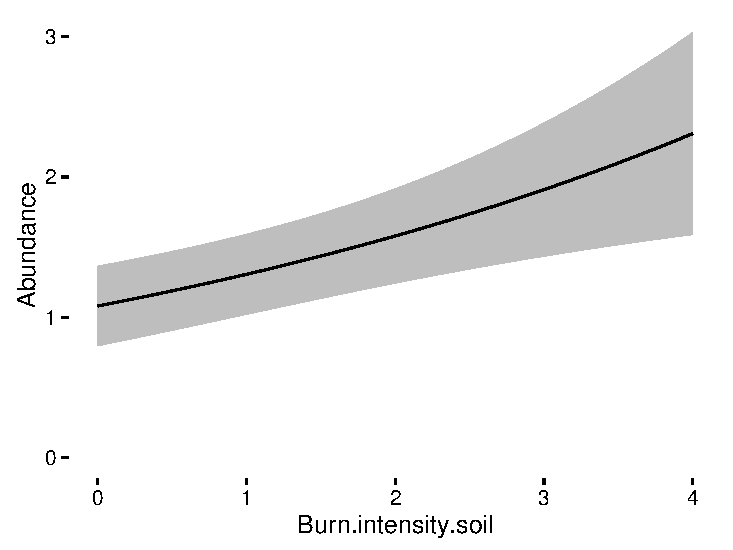
\includegraphics{diversityocc_files/figure-latex/unnamed-chunk-16-1} \end{center}

\end{CodeChunk}

\subsection{Model selection for alpha diversity
modeling}\label{model-selection-for-alpha-diversity-modeling}

\section{Discussion}\label{discussion}

The \pkg{DiversityOccupancy} package lets scientists and managers take
dessitions based on species information, diversity information or both.
In some countries, laws require that the decision is taken based on
endangered species information, the possibility on selecting an area, or
manage environments based on both diversity and species specific
information, gives a possibility to managers or decision makers wanting
to use diversity with laws requiring them to take species into account.

\renewcommand\refname{References}
\bibliography{Derek}


\end{document}

